\documentclass[12pt, twoside]{article}
\usepackage[letterpaper, margin=1in, headsep=0.5in]{geometry}
\usepackage[english]{babel}
\usepackage[utf8]{inputenc}
\usepackage{amsmath}
\usepackage{amsfonts}
\usepackage{amssymb}
\usepackage{tikz}
\usepackage{yhmath}
%\usetikzlibrary{quotes, angles}

\usepackage{graphicx}
\usepackage{enumitem}
\usepackage{multicol}

\usepackage{fancyhdr}
\pagestyle{fancy}
\fancyhf{}
\renewcommand{\headrulewidth}{0pt} % disable the underline of the header

\fancyhead[RE]{\thepage}
\fancyhead[RO]{\thepage \\ Name: \hspace{3cm}}
\fancyhead[L]{BECA / Dr. Huson / 10th Grade Geometry\\* 8 May 2019}

\begin{document}
\subsubsection*{10.10 Do Now: Volume, density, trig review}
 \begin{enumerate}
    \item Sarah needs to replace two concrete sections in her sidewalk, as modeled below. Each section is 36 inches by 36 inches and 4 inches deep.\\[0.5cm]
    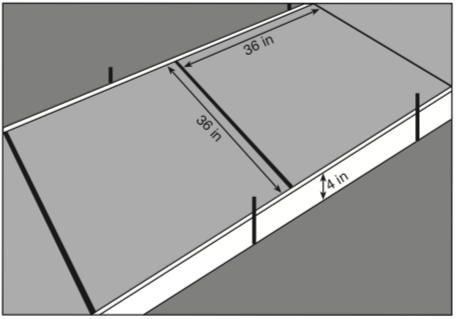
\includegraphics[width=0.5\textwidth]{walk_Aug2018-31.png}
      \begin{enumerate}
        \item Determine and state the volume of concrete needed, \emph{in cubic feet}. \vspace{1cm}
        \item Sarah can mix her own concrete for \$3.25 per cubic foot. How much money will it cost her to replace the two concrete sections?
    \end{enumerate} \vspace{2.5cm}

    \item The greenhouse pictured below can be modeled as a rectangular prism with a half-cylinder on top. The rectangular prism is 20 feet wide, 12 feet high, and 45 feet long. The half-cylinder has a diameter of 20 feet.\\[0.5cm]
    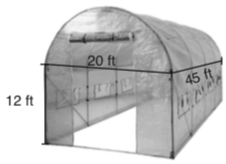
\includegraphics[width=0.3\textwidth]{greenhouse_Jun2018-7.png}\\
    To the \emph{nearest cubic foot}, what is the volume of the greenhouse?

\newpage
  \item In a right triangle, the acute angles have the relationship $\sin (2x+4)=\cos(46)$.\\[0.25cm]
    What is the value of x? \vspace{3cm}

  \item If $\sin (2x-11)^\circ = \cos(4x+11)^\circ$, what is the value of $x$? \vspace{3cm}


  \item In the model below, a support wire for a telephone pole is attached to the pole and anchored to a stake in the ground 15 feet from the base of the telephone pole. Sachem places a 6-foot wooden pole under the support wire parallel to the telephone pole, such that one end of the pole is on the ground and the top of the pole is touching the support wire. He measures the distance between the bottom of the pole and the stake in the ground.\\[0.5cm]
    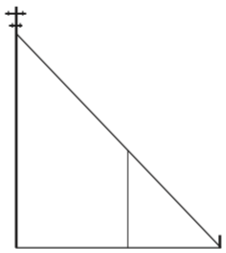
\includegraphics[width=0.3\textwidth]{pole_Aug2018-29.png}\\
  Sachem says he can approximate how high the support wire attaches to the telephone pole by using similar triangles. Explain why the triangles are similar.


  \end{enumerate}
  \newpage
  \setcounter{page}{1}
\subsubsection*{10.10 Classwork: Cross sections and 3-dimensional rotations}
 \begin{enumerate}

   \item A bakery sells hollow chocolate spheres. The larger diameter of each sphere is 4 cm. The thickness of the chocolate of each sphere is 0.5 cm. Determine and state, to the nearest tenth of a cubic centimeter, the amount of chocolate in each hollow sphere.\\[0.5cm]
   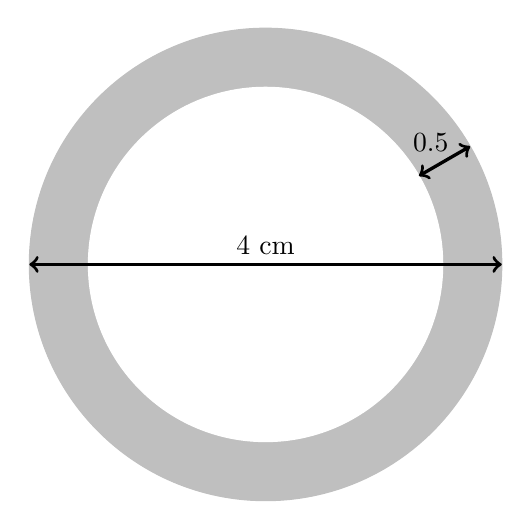
\begin{tikzpicture}[scale=1.5]
     \draw [fill, color=lightgray] (0,0) circle[radius=2];
     \draw [fill, color=white] (0,0) circle[radius=1.5];
     \draw [very thick, <->] (0:2)--(180:2);
     \draw (0,0) node[above]{$4$ cm};
     \draw [very thick, <->]  (30:1.5)--(30:2);
     \draw (32:1.65) node[above]{$0.5$};
   \end{tikzpicture}


   \item As shown in the diagram below, the radius of a cone is 2.5 cm and its slant height is 6.5 cm.\\[0.5cm]
     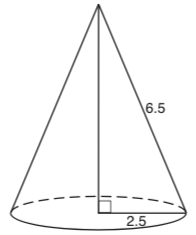
\includegraphics[width=0.25\textwidth]{cone_Jan2019-23.png}
     \begin{enumerate}
       \item Find the height of the cone. \vspace{1cm}
       \item How many cubic centimeters are in the volume of the cone? Express your answer in terms of $\pi$.
   \end{enumerate} \vspace{2.5cm}

  \item Which three-dimensional figure will result when a rectangle 6 inches long and 5 inches wide is continuously rotated about the longer side?
    \begin{enumerate}
      \item a rectangular prism with a length of 6 inches, width of 6 inches, and height of 5 inches
      \item a rectangular prism with a length of 6 inches, width of 5 inches, and height of 5 inches
      \item a cylinder with a radius of 5 inches and a height of 6 inches
      \item a cylinder with a radius of 6 inches and a height of 5 inches
    \end{enumerate}

  \item An isosceles right triangle whose legs measure 6 is continuously rotated about one of its legs to form a three-dimensional object. The three-dimensional object is a
    \begin{enumerate}
      \item cylinder with a diameter of 6
      \item cylinder with a diameter of 12
      \item cone with a diameter of 6
      \item cone with a diameter of 12
    \end{enumerate}

    \item A right cylinder is cut perpendicular to its base. The shape of the cross section is a
      \begin{enumerate}
        \item circle
        \item cylinder
        \item rectangle
        \item triangular prism
      \end{enumerate}

    \item A homeowner is building three steps leading to a deck, as modeled by the diagram below. All three step rises, $\overline{HA}$,  $\overline{FG}$, and  $\overline{DE}$, are congruent, and all three step runs, $\overline{HG}$,  $\overline{FE}$, and  $\overline{DC}$, are congruent. Each step rise is perpendicular to the step run it joins. The measure of $\angle CAB = 36^\circ$ and $\angle CBA = 90^\circ$.\\[0.5cm]
      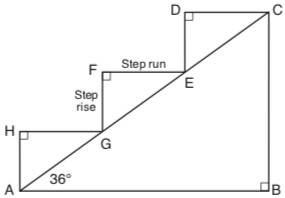
\includegraphics[width=0.4\textwidth]{steps_Aug2018-33.png}\\
    If each step run is parallel to $\overline{AB}$ and has a length of 10 inches, determine and state the length of each step rise, to the \emph{nearest tenth of an inch}.\\[3cm]
    Determine and state the length of $\overline{AC}$, to the \emph{nearest inch}.

\end{enumerate}
\end{document}

\item A bakery sells hollow chocolate spheres. The larger diameter of each sphere is 4 cm. The thickness of the chocolate of each sphere is 0.5 cm. Determine and state, to the nearest tenth of a cubic centimeter, the amount of chocolate in each hollow sphere.\\
The bakery packages 8 of them into a box. If the density of the chocolate is 1.308 g/$\mathrm{cm}^3$, determine and state, to the nearest gram, the total mass of the chocolate in the box.
